\documentclass[11pt,english]{toptesi}

%%%%%%%%%%%%%%%%%%%%%%%%%%%%%%%%%%%%%%%%%%%%%%%%%%%%%%%%%%%%%%%

\usepackage[utf8]{inputenc} %utf8
\usepackage[english]{babel}
\usepackage[T1]{fontenc}
\usepackage{blindtext}
\usepackage{graphicx,wrapfig}
\usepackage{booktabs}
\usepackage{lmodern}
\usepackage{varioref}
\usepackage{url}
\usepackage{array}
\usepackage{paralist}{\obeyspaces\global\let =\space}
\usepackage{verbatim}
\usepackage{subfig}
\usepackage{tabularx}
\usepackage{amsmath}
\usepackage{amsfonts}
\usepackage{float}
\usepackage{amssymb}
\usepackage{multicol}
\usepackage{multirow}
\usepackage{listings}
\usepackage[pass]{geometry}
\usepackage[figuresright]{rotating}
\usepackage{algorithm}
\usepackage{algorithmic}
\usepackage{amsmath}
\usepackage[babel]{csquotes}
\usepackage{hyperref}
\usepackage[backend=bibtex]{biblatex}

%aggiunti da Seb
\usepackage{dirtytalk}
\usepackage{mathtools}
\usepackage{tikz} % per i grafici
\usepackage{tikz-3dplot}
\newcommand\todo[1]{\textcolor{red}{[TODO:#1]}}
\usepackage{fancyvrb}
\def\changemargin#1#2{\list{}{\rightmargin#2\leftmargin#1}\item[]}
\let\endchangemargin=\endlist
%%%%%%%%%%%%%%%%%%%%%%%%%%%%%%%%%%%%%%%%%%%%%%%%%%%%%%%%%%%%%%%

% CONFIGURAZIONE LINK E RIFERIMENTI
\hypersetup{%
    pdfpagemode={UseOutlines},
    bookmarksopen,
    pdfstartview={FitH},
    colorlinks,
    linkcolor={black}, %COLORE DEI RIFERIMENTI AL TESTO
    citecolor={black}, %COLORE DEI RIFERIMENTI ALLE CITAZIONI
    urlcolor={black} %COLORI DEGLI URL
}

%%%%%%%%%%%%%%%%%%%%%%%%%%%%%%%%%%%%%%%%%%%%%%%%%%%%%%%%%%%%%%%

% CONFIGURAZIONE LISTATI/CODICE - CANCELLARE SE NON NECESSARIO
% PYTHON - BIANCO E NERO

\lstset{%
	captionpos=b,
	language=Matlab,
	basicstyle =\small\fontfamily{pcr},
	keywordstyle=\color{black}\bfseries,
	breaklines=true,
	breakatwhitespace=true,
	showstringspaces=false,
	frame=lines,
	numbers=left,
	numberstyle=\footnotesize,
	morekeywords={subs, simplify, genforces, solve, functionalDerivative, matlabFunction}
}
%%%%%%%%%%%%%%%%%%%%%%%%%%%%%%%%%%%%%%%%%%%%%%%%%%%%%%%%%%%%%%%
% CONFIGURAZIONE GRAFICI
\usetikzlibrary{calc,3d}
%%%%%%%%%%%%%%%%%%%%%%%%%%%%%%%%%%%%%%%%%%%%%%%%%%%%%%%%%%%%%%%

% FRENCHSPACING ABILITATO - CANCELLARE PER SPAZIATURA ALL'INGLESE
%\frenchspacing

%%%%%%%%%%%%%%%%%%%%%%%%%%%%%%%%%%%%%%%%%%%%%%%%%%%%%%%%%%%%%%%

%DEFINIZIONE SEZIONI IN NUMERAZIONE ROMANA
%ELENCO DEI LISTATI/CODICI
\makeatletter
\newcommand\listofcodes{%
 \iffrontmatter\else\frontmattertrue\fi
 \if@openright\cleardoublepage\else\clearpage\fi
 % change the meaning of \chapter in a group
 \begingroup\def\chapter##1{\@schapter}
 \phantomsection % for the hyperlink
 \lstlistoflistings
 \endgroup
}
\makeatother

%%%%%%%%%%%%%%%%%%%%%%%%%%%%%%%%%%%%%%%%%%%%%%%%%%%%%%%%%%%%%%%

% METADATI PDF
\pdfinfo{%
  /Title    (Control oriented modelling of four wheeled electric vehicles)
  /Author   (Sebastian Giles)
  /Subject  (How to write meaningful titles)
  /Keywords (LaTeXi foo bar baz meaningful PIT Presicce)
}

%%%%%%%%%%%%%%%%%%%%%%%%%%%%%%%%%%%%%%%%%%%%%%%%%%%%%%%%%%%%%%%
% FRONTESPIZIO (template non permette riordinamento?)

% UNIVERSITA - NOME
\ateneo{Università Politecnica delle Marche}
% FACOLTA - DICITURA
\FacoltaDi{Faculty of }
% FACOLTA - NOME
\facolta{Engineering}

% CORSO DI LAUREA - DICITURA (MANTENERE LO SPAZIO)
\CorsoDiLaureaIn{Bachelor of Science in }
% CORSO DI LAUREA - NOME
\corsodilaurea{Computer and Automation Engineering}

% TIPOLOGIA TESI
\TesiDiLaurea{Bachelor's Thesis}

% TITOLO
\titolo{Control oriented modelling of four wheeled electric vehicles}

% SOTTOTITOLO
%\sottotitolo{Il titolo è già lungo di suo no?}

% LOGO UNIVERSITA
\logosede{images/logo}

% RELATORE/I - DICITURA
\AdvisorName{Advisor}
% RELATORE - PROF. NOME E COGNOME
\relatore{prof.\ Andrea Bonci}
% RELATORE AGGIUNTIVO - PROF NOME E COGNOME
% SE SI HA SOLO UN RELATORE ELIMINARE E CAMBIARE Advisors in Advisor
%\secondorelatore{prof.\ Neo Cortex}

% CANDIDATO - DICITURA (MANTENERE I DUE PUNTI)
\CandidateName{Candidate:}
% SECONDO CANDIDATO - ELIMINARE O DECOMMENTARE
%secondocandidato{Bombo de Bombis}

% CANDIDATO - NOME E COGNOME
\candidato{Sebastian Nicolas Giles}

% DATA - MESE ANNO
\sedutadilaurea{July 2018}

%%%%%%%%%%%%%%%%%%%%%%%%%%%%%%%%%%%%%%%%%%%%%%%%%%%%%%%%%%%%%%%

% LISTA DEI CAPITOLI DA INCLUDERE
% VIENE FATTO DOPO, QUI A CHE SERVE? (commentata e ancora va)
% \includeonly{%
% 01-intro,%
% 02-stuff,%
% 03-conclusion,%
% 04-appendix-A,%
% }

% FILE DI BIBLIOGRAFIA
\bibliography{bibliography}

%%%%%%%%%%%%%%%%%%%%%%%%%%%%%%%%%%%%%%%%%%%%%%%%%%%%%%%%%%%%%%%

% INIZIO DOCUMENTO
\begin{document}
\english

\frontespizio

%%%%%%%%%%%%%%%%%%%%%%%%%%%%%%%%%%%%%%%%%%%%%%%%%%%%%%%%%%%%%%%

%INTERLINEA - DEFAULT 1 - NON ESAGERATE, NON SUPERATE MAI 1.3 ;)
%LO DICI TE, qui mi pare che le tesi siano tutte spaziatissime...
\interlinea{1.3}

%%%%%%%%%%%%%%%%%%%%%%%%%%%%%%%%%%%%%%%%%%%%%%%%%%%%%%%%%%%%%%%

\frontmatter

% % DEDICA - PERSONALIZZARE
% % VSPACE - PROPORZIONE USATA PER CENTRATURA VERTICALE DEL TESTO
% % FLUSHRIGHT - ALLINEAMENTO ORIZZONTALE A DESTRA
% \vspace*{\stretch{1}}
% \begin{flushright}
% \noindent
% Dedicato a qualcuno
% \end{flushright}
% \vspace*{\stretch{6}}
% \cleardoublepage
%
% % CITAZIONE - PERSONALIZZARE
% % VSPACE - PROPORZIONE USATA PER CENTRATURA VERTICALE DEL TESTO
% % FLUSHRIGHT - ALLINEAMENTO ORIZZONTALE A DESTRA
% \vspace*{\stretch{1}}
% \begin{flushright}
% \noindent
% Citazione
% \textit{Qualcuno}
% \end{flushright}
% \vspace*{\stretch{6}}
% \cleardoublepage

%%%%%%%%%%%%%%%%%%%%%%%%%%%%%%%%%%%%%%%%%%%%%%%%%%%%%%%%%%%%%%%

% RINGRAZIAMENTI - PERSONALIZZARE
\ringraziamenti
Thanks to someone

%%%%%%%%%%%%%%%%%%%%%%%%%%%%%%%%%%%%%%%%%%%%%%%%%%%%%%%%%%%%%%%

% ABSTRACT - PERSONALIZZARE
\sommarioITA
I motori elettrici non contengono parti mobili all'infuori dell'assieme dell'albero motore, questo li rende più compatti e più semplici rispetto a motori termici di prestazioni simili. L'utilizzo di più motori per la trazione dei veicoli è quindi fattibile senza incorrere in eccessivo peso o complessità. L'Utilizzo di un motore per ogni ruota motrice può ridurre peso, dimensioni e complessità della trasmissione. Questo è dato dall'assenza dei differenziali e dal fatto che la potenza meccanica possa essere prodotta più vicino alle ruote.

I motori possono inoltre essere controllati individualmente per produrre coppie differenti, risultando in un momento di rotazione attorno all'asse verticale, questa strategia di controllo è chiamata torque vectoring.
Il torque vectoring può essere usato per corregere una vettura sovrasterzante o sottsterzante, migliorando la sicurezza dei veicoli stradali e la maneggevolezza di auto da competizione.
Il controllo della trazione è inoltre ottenibile indipendentemente per ogni ruota, permettendo di percorrere curve a velocità maggiori.

L'obiettivo di questo studio è la derivazione di un modello matematico utilizzabile in simulazione e per lo sviluppo di controllori per il torque vectoring e il controllo della trazione nei veicoli elettrici.

L'interesse per lo sviluppo del modello è sorto in vista di una prossima partecipazione alle competizioni di Formula Student Electric. Il modello è quindi concepito per applicazioni competitive. L'alta rigidezza sospensiva, diffusa nelle vetture che competono in queste competizioni, è stata tenuta in considerazione per ottenere alcune approssimazioni.

La modellazione delle dinamiche di rollio rende prevedibili i transitori di trasferimento di carico, garantendo maggiore precisione durante le manovre a frequenza più alta come i cambi di corsia, le piccole chicane e gli stretti slalom che tipicamente compongono i percorsi degli eventi di Autocross ed Endurance in Formula Student.
L'inclusione del comportamento di beccheggio e rollio permette anche di studiare la correlazione tra i trasferimenti di carico e l'escursione delle sospensioni, essendo quest'ultima una grandezza fisica facilmente misurabile in tempo reale e quindi utilizzabile come ingresso al sistema di controllo del veicolo.
Le dinamiche di sterzo posteriori sono incluse nel secondo modello presentato poichè il regolamento Formula Student permette esplicitamente l'utilizzo di quattro ruote sterzanti e la modellazione non ha richiesto alcun impegno aggiuntivo.

Il capitolo \ref{chap:6dof} descrive fisicamente un modello a sei gradi di libertà, successivamente ne viene fornita la formulazione lagrangiana. Nel capitolo \ref{chap:12dof} il modello viene esteso con 6 gradi di libertà aggiuntivi per la descrizione della rotazione delle ruote e delle dinamiche di sterzo anteriore e posteriore.

La formulazione lagrangiana è stata costruita simbolicamente utilizzando la  MATLAB Symbolic Math Toolbox per facilitare le derivate e le trasformazioni di coordinate.
Sono state scritte delle funzioni per risolvere algebricamente le equazioni di Lagrange e fornire una rappresentazione in spazio di stato del sistema.
Tutti gli script sono scritti in forma vettoriale rendendo il codice più compatto e leggibile
Le simulazioni sono state eseguite in ambiente simulink, in cui i due modelli matematici ottenuti sono stati implementati in forma modulare, accompagnati da un modello empirico per le forze di attrito generate dagli pneumatici.
L'utilizzo di un'animazione 2D della vettura ha facilitato la risoluzione dei problemi rendendo più intuibile il siginificato dei risultati numerici.


\sommario
The use of multiple motors to independently drive each wheel of a road vehicle allows for handling and safety improvements by means of electronic control systems.
In this work a 6DoF mathematical model of the four wheeled car is developed to be used in control system design. It includes longitudinal and lateral load transfer dynamics. The model is then extended to include the dynamic effects of the wheels and the steering system.
The model is derived using Lagrangian mechanics with the help of the MATLAB Symbolic Math Toolbox.
This work also describes the method used for simulations and tests in the Simulink software environment.
%%%%%%%%%%%%%%%%%%%%%%%%%%%%%%%%%%%%%%%%%%%%%%%%%%%%%%%%%%%%%%%

% INDICI - ELIMINARE GLI INDICI NON NECESSARI

% INDICE GENERALE
\tableofcontents

% INDICE DELLE FIGURE
\listoffigures

% INDICE DELLE TABELLE
% \listoftables

% INDICE DEI CODICI
%\listofcodes

%%%%%%%%%%%%%%%%%%%%%%%%%%%%%%%%%%%%%%%%%%%%%%%%%%%%%%%%%%%%%%%

\mainmatter

% INCLUSIONE FILE CAPITOLI - PERSONALIZZARE - TENERE COERENTE CON LISTA IN ALTO
% ma la lista in alto l'ho esclusa
\chapter{Introduction}
\label{chap:intro}
\section{Background}
\label{sec:background}

\section{Objectives}
\label{sec:objectives}

\section{Approach}
\label{sec:approach}

\chapter{Tyres}
\label{chap:tyres}
Tyres are the main source of external forces and moments acting upon any road vehicle\todo{cita milliken race car VD}, for this reason, understanding their behaviour is key in making accurate predictions about vehicle dynamics. The tyre is a very complex system exhibiting high non linearities, especially in the wide operating range imposed by racing\todo{trova una fonte}.
A realistic model of the road-vehicle interaction is clearly necessary in order to obtain significant results from simulations but the detailed study of tyres is far beyond the objectives of this work.
The present chapter provides only the fundamental concepts behind tire modelling needed to introduce the numerical model that was used.
\section{Tyre modelling basics and definitions}
\label{sec:tyrebasics}
All forces acting between the vehicle and the road are distributed over the surfaces of the so called \textit{tyre contact patches}. As the tyre contact patches size and shape are dependent on the operating conditions \todo{trova fonte}, for each wheel, we consider a \textit{tyre contact point}, $C$, as the point at which an applied vector can approximate all forces acting between the tyre and the road.

Various definitions for this point may be used to include more or less complicated effects due to tyre compliance, such as dynamic caster or centrifugal deformation.\todo{cita un articolo su questi effetti}
Modelling of such phenomena would require extensive experimental data and is considered to be outside the scope of this research, thus, the following simplified definition for the tyre contact point was deemed satisfactory. The road is assumed to be a flat and planar surface and the tyre is to be considered as an infinitely thin rigid disk tangent to this plane.  The tangent point will be considered as the tyre contact point.

The wheel co-ordinate system is required for the definition of all the related physical quantities.
We consider a reference system \todo{figura} with origin in $C$, whose $x$ axis lies along the intersection between the road plane and the wheel plane, such that it is generally oriented in the direction of motion, and whose $z$ axis is pointing down, perpendicular to the road plane, the $y$ axis is determined by asserting $Cxyz$ to be a right-handed cartesian coordinate system.

The angle between the $xz$ plane and the tyre plane is known as the camber angle \todo{trova definizione SAE}.

The $x$, $y$ and $z$ axes are respectively associated with the \textit{longitudinal}, \textit{lateral} and \textit{vertical} dimensions of the wheel.

As tyre compliance is neglected in this work, the vertical force $F_z$ acting through the tyre and its contact point is considered as indipendent of tyre behaviour. This choice also excludes all transient responses of the rubber. The longitudinal and lateral friction forces, $F_x$ and $F_y$, are to be computed since these are what effectively make the vehicle accelerate and corner and are of primary interest.

Consider a wheel \todo{figura} having radius $R$ and angular velocity $\omega$ about it's spin axis, passing through the wheel center and orthogonal to the wheel plane.
We consider $\omega$ as positive when the upper half of the wheel is moving in the positive $x$ direction. The lowest point of the wheel is then moving with velocity $v_{w} = -\omega R$ in the wheel $x$ direction.
By considering the velocity vector of the point $C$ in a road-fixed reference system and letting $v_x$ and $v_y$ be its components along the wheel $x$ and $y$ axes the longitudinal velocity of the road with respect to the wheel system is $v_{rx} = - v_x$.
It is therefore possible to define the longitudinal slip as the difference between these two velocities at the contact point:
$$v_{sx} = v_{w} - v_{rx} = v_x - \omega R .$$

We further define the slip ratio as \todo{SAE J670}
$$ \kappa = - \frac{v_{sx}}{v_{x}} = \frac{\omega R}{v_x}-1.$$
The slip angle $\alpha$ is the angle formed between the contact point velocity vector in the road frame and the wheel $x$ axis. It can be formally defined by the equation
$$\tan{\alpha} = \frac{v_y}{v_x}.$$

$F_x$ and $F_y$ scale almost linearly with the vertical load exerted on the tyre, for this reason it makes sense to define the longitudinal and lateral friction coefficients as
$$ \mu_x = \frac{F_x}{F_z}$$
and
$$ \mu_y = \frac{F_y}{F_z}$$
$\kappa$ and $\alpha$ are the primary variables affecting the friction coefficients and are used to estimate $\mu_x$ and $\mu_y$. However, there are other factors that define the steady state tyre behaviour, some of which are relatively straight-forward, such as camber angle, vertical load, wheel rotational velocity, tyre pressure and temperature and others which are extremely difficult to quantify, such as asphalt characteristics, and rubber aging.

The typical correlation between friction coefficients and slip ratio and slip angle is shown in
\todo{figure dei coeff di attrito tipo dal Kiencke}
, ideally, all curves pass through the origin, due to the fact that without slip the speed of the wheel is the same as that of the contact point, and no friction forces can be generated. In reality, there is a slight offset caused by rolling resistance and asymmetric tyre contructions \todo{letto in qualcosa di pacejka}.

It is also clearly noticeable that in order to obtain maximum longitudinal traction their will be an optimal amount of slip ratio. Limiting the tractive torque to not exceed this value is the exact purpouse of launch control systems.

Another effect of the pneumatic tyre is the so called self aligning torque, this moment is exerted about the tyre $z$ axis and is an important contributor to the steering effort which is applied to the steering wheel, this will be relevant to the steering dynamics introduced in the 12 DoF model presented in Chapter \ref{chap:12dof}.

\section{Magic Formula tyre models}
\label{sec:mf}
A series of semi-empirical tyre models was developed during the past 30 years by Hans B. Pacejka of Delft University.

These models are based on the same parametric mathematical expression, nicknamed \textit{Magic Formula} because of the good fitting properties it offers despite the lack of a physical foundation. The general form of these functions is
$$ R(k) = d\sin(c\arctan(b(1-e)k+e\arctan(bk))) $$
where $R$ is the physical quantity to be estimatated and $k$ is the most relevant variable whilst $d$, $c$, $b$, $e$ and $k$ are fitting coefficients, which may in turn depend on other variables.
The set of equations released in 1996, called \textit{Deft Tyre 96} \todo{riferisci all'articolo 96} was the first to include combined effects of longitudinal and lateral slip, subsequent editions of the model have been conceived to model tyre pressure changes \todo{riferisci all'articolo 2004} and more.
The version which has been chosen in this work is the PAC2002 model \todo{riferisci all'URL del pdf online}, formalized by MSC Software and released as part of their Adams CAR multibody simulation package, which includes a set of tools for obtaining the fitting coefficients from experimental datasets. The standard file format used for the storage of the tyre coefficients is text based and can also be interpreted by an appropriate MATLAB script \todo{refer to implementation paragraph}.
The input variables of this tyre model are the slip ratio, slip angle, vertical force and camber angle. Outputs are the longitudinal and lateral forces and the self aligning torque.

\section{Tyre Data}
\label{sec:tyredata}

Experimental tyre data that is specific to Formula SAE and Formula Student tyres has been gathered by the FSAE Tyre Test Consortium \todo{link al TTC} at the Calspan test facility. The expensive tests are funded by the one-time fee the student teams pay to access the information.
As access to experimental data was not possible during the preparation of this work, a sample tyre model was used. As the coefficients were given, the fitting process was not necessary.
To verify that the tyre model was consistent with the physical intuitions developed so far, some plots were drawn (shown in \todo{figure fatte in matlab}), these both exhibit a plausible correlation between the slip quantities and the friction forces.

%\chapter{Common models}
\label{chap:stateoftheart}
\section{Single Track Model}
\label{sec:singletrack}
\section{\textit{some other model}}
\label{sec:modeltwo}

\chapter{Six degree-of-freedom vehicle model}
\label{chap:6dof}
\section{6DoF Model structure}
\label{sec:6dofconcept}
The state of the car is identified by the six degrees of freedom required to define the position and orientation of its chassis. The car interacts with the road through a simplified suspension system.
The model outputs are the vertical forces on each of the four wheels and the velocities of the respective ground contact points, which may be used to calculate friction by an external tyre model.
Inputs to the model are the longitudinal and lateral forces acting on each wheel and the steering angle. The latter effectively rotates the force vectors of the front wheels allowing direction control.
The block diagram in figure \ref{6flow} shows the intended flow of information for this model working in conjuction with a tyre model.
\begin{figure}[ht]
  \centering
  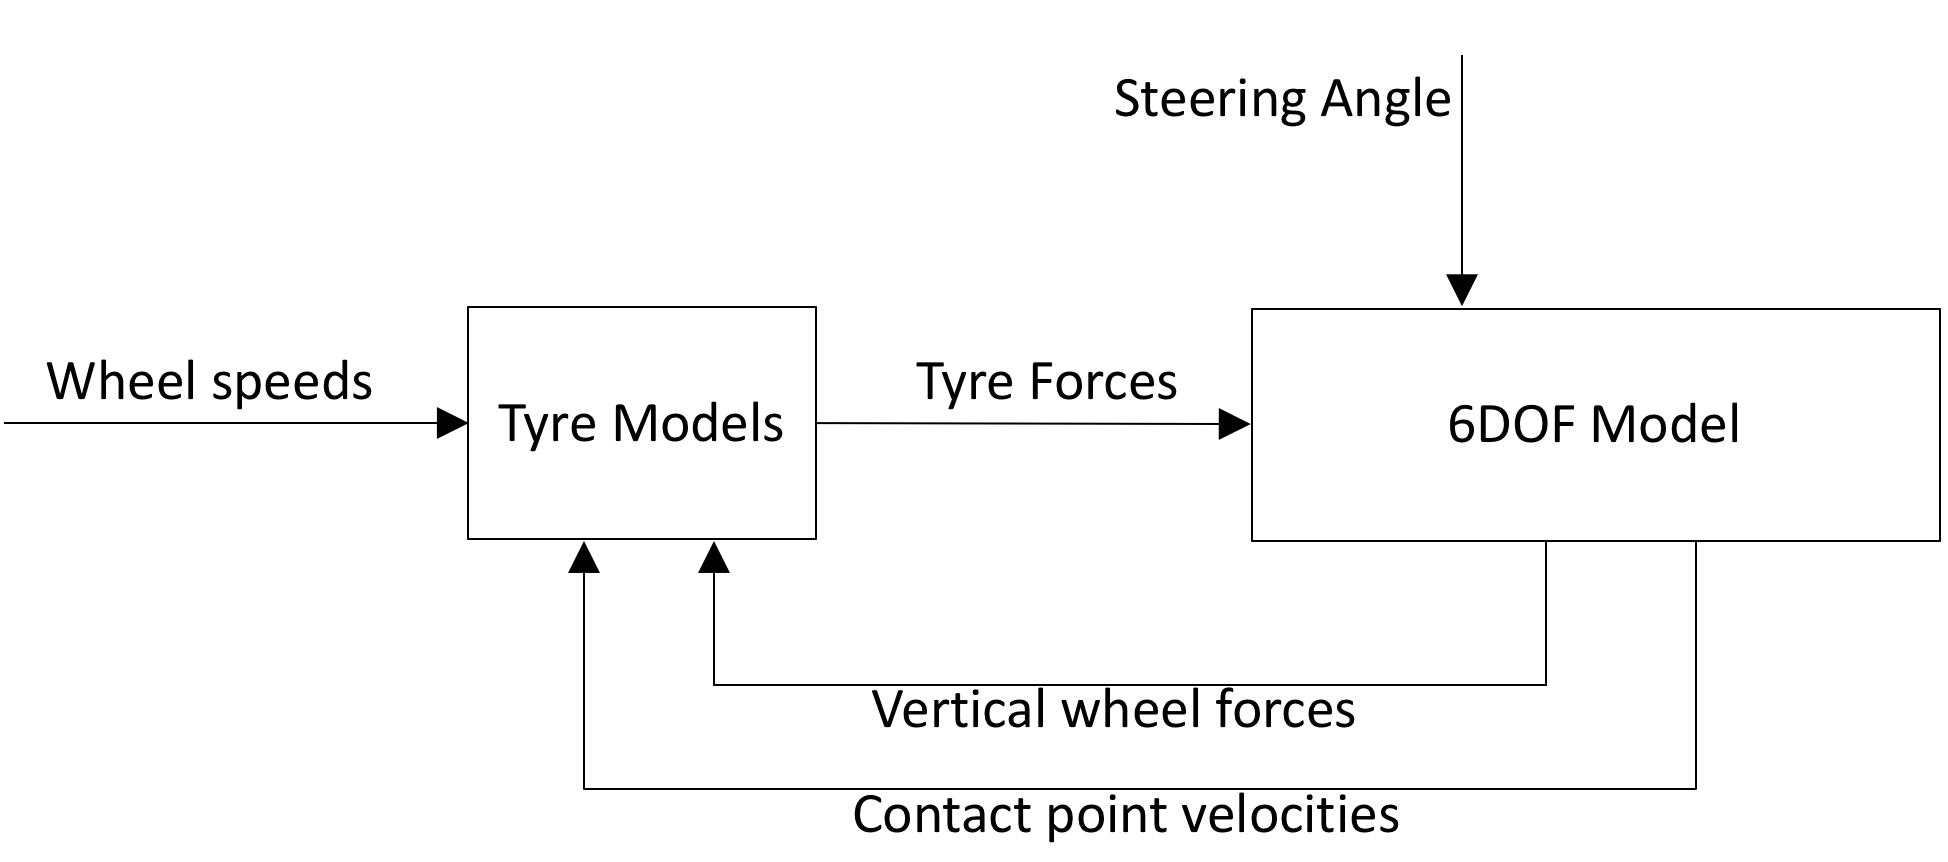
\includegraphics[width=\textwidth]{images/6flow.png}
  \caption{Information flow between the tyre model and the 6dof vehicle model.}
  \label{6flow}
\end{figure}
\section{Chassis description}
\label{sec:body}
The road is assumed to be a horizontal plane. In the $xyz$ inertial reference system $z$ is pointed downwards, in the direction of gravity whilst $x$ and $y$ lye on the road surface and may be arbitrarily chosen as long as the right-handedness of the reference frame is guaranteed.

The chassis is represented by a rigid body whose mass $m$ and rotational inertia matrix $I$ resemble those of the entire vehicle, inclusive of the driver and the wheels.

The body reference system $x'y'z'$ is fixed to the chassis and originates at the Center of Gravity. An unambiguous definition of the axes is made in the static equilibrium orientation when the suspension system is bearing the weight of the car and no other forces are at play (this will be later referenced as the \textit{resting condition}). In this condition $z'$ is defined to be parallel to $z$ and likewise pointed downwards, $x'$ is directed forwards, parallel to the road plane, and the $y'$ axis is oriented to the right of the car as seen by the driver. The chassis reference system here defined is in line with the SAE J670 definition depicted in figure \ref{saeaxes}.
\begin{figure}[ht]
  \centering
  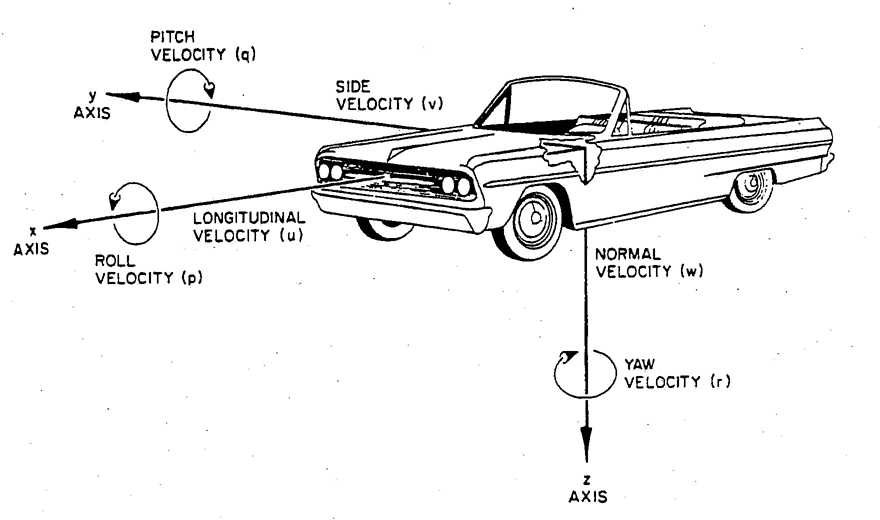
\includegraphics[height = 7cm]{images/saeaxes}
  \caption{The chassis reference system as defined in the SAE J670 standard.}
  \label{saeaxes}
\end{figure}

The attitude of the chassis is defined by the Tait-Bryan angles mapping the inertial system axes to the chassis axes \todo{appendix}. Note that the given definition for the chassis reference system implies zero roll and pitch at static equilibrium.

The chassis is assumed to be symmetrical about the $x'z'$ plane, this identifies the $y'$ axis as a principle axis of inertia and eliminates all the related product of inertia terms from the inertia matrix evaluated in the chassis reference system.
$$
I = \begin{bmatrix}
I_{xx} & 0      & I_{xz}\\
0      & I_{yy} & 0     \\
I_{xz} & 0      & I_{zz}
\end{bmatrix}.
$$

\section{Suspension}
\label{sec:suspension}
Suspension is represented by four vertical linear spring-damper systems associated with each wheel of the car. Quantities relating to each of the systems will be distinguished by subscripts according to Table \ref{table:subscripts}, the $w$ subscript is used when referring generically to any one of them.

\begin{table}[ht]
  \caption{Wheel and suspension systems subscripts} % title of Table
  \centering % used for centering table
  \begin{tabular}{l l l l} % left aligned columns (4 columns)
    \hline\hline %inserts double horizontal lines
    Subscript & Pertaining wheel or suspension system \\ [0.5ex] % inserts table
    %heading
    \hline % inserts single horizontal line
    $FR$ & Front Right \\ % inserting body of the table
    $FL$ & Front Left \\
    $RR$ & Rear Right \\
    $RL$ & Rear Left \\ [1ex] % [1ex] adds vertical space
    \hline %inserts single line
  \end{tabular}
  \label{table:subscripts} % is used to refer this table in the text
\end{table}

The upper end of each suspension system is attached to an appropriate point $P_w$ statically defined with respect to the chassis, the lower end point is obtained by projecting $P_w$ onto the road plane.
The spring length $h_w$ is given by the distance between $P_w$ and the road plane, so it is equal to the opposite of the inertial system $z$ coordinate of $P_w$.

\begin{figure}[ht]
  \centering
  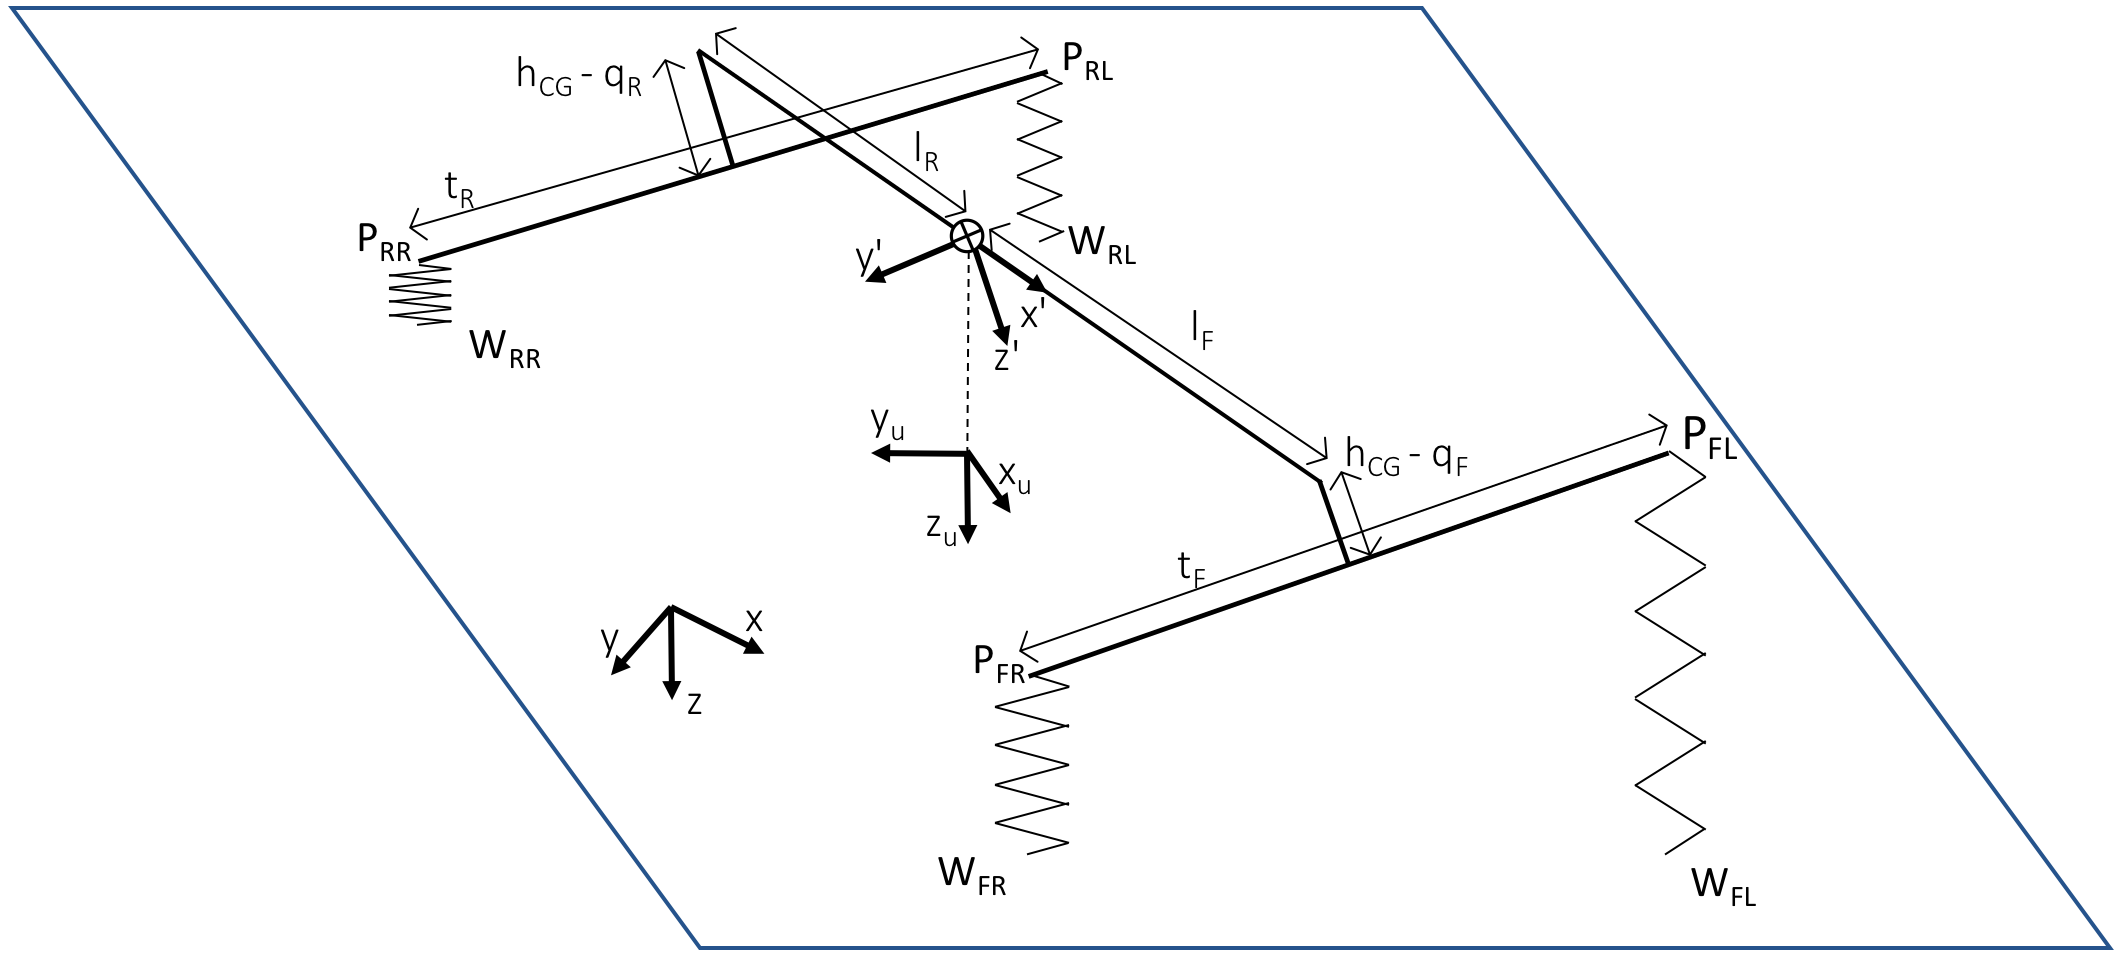
\includegraphics[width=\textwidth]{images/3dview}
  \caption{Description of the 6 DoF model geometry.}
  \label{3dview}
\end{figure}

The correct weight transfer effects are obtained by assigning the corresponding wheel contact point $x$ and $y$ coordinates to each of the $P_w$ points, these are easily calculated from the front and rear track lengths ($t_F$ and $t_R$) and the distances of the front and rear axles from the CoG ($l_F$ and $l_R$).

The $z$ co-ordinates of the $P_w$ points with respect to the chassis system are finally chosen in order to obtain realistic roll dynamics.

Automotive suspension systems can be characterized by a roll center for each axle. This is the point at which lateral forces acting on the wheels are reacted to the chassis.
The roll center is usually below the center of mass, causing vehicles to lean towards the outside of turns when driving, this is in line with the situation shown in figure \ref{roll}, where the lateral force at the center of mass is the centrifugal force acting in the non inertial reference frame of the car, balanced by friction acting on the wheel contact points.

\begin{figure}[ht]
  \centering
  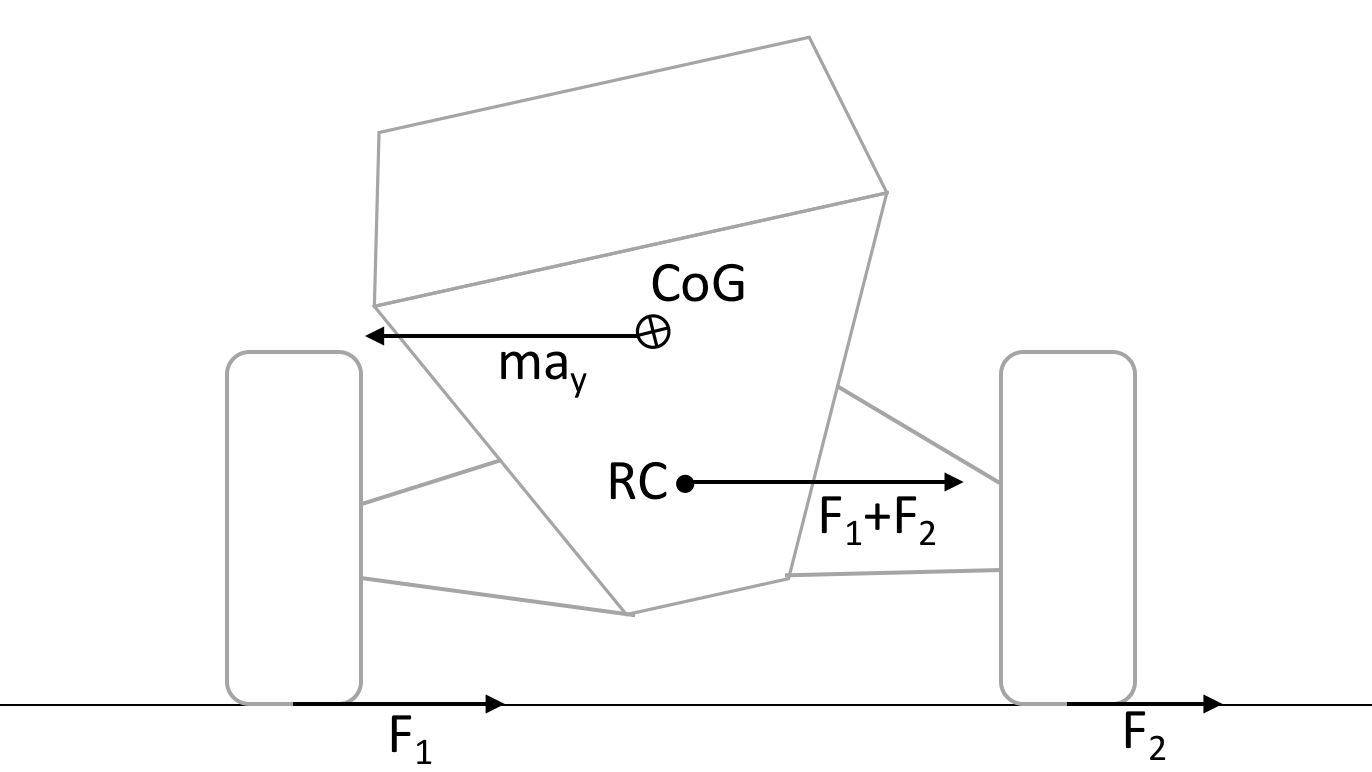
\includegraphics[height = 7cm]{images/roll}
  \caption{Body roll during cornering.}
  \label{roll}
\end{figure}

The roll center height, as defined by the SAE in J670, is determined by suspension kinematics and dynamic load distribution so it is almost never constant.
In the developed model, each roll center is approximated by the midpoint of the left and right $P_w$ points of the corresponding axle. Appendix \ref{chap:roll} justifies this approximation.

The roll center heights ($q_F$ and $q_R$) are a common design specification in race cars.
Their values can be obtained by means of multibody simulation, experimental tests or kinematic approximations.
$q_F$ and $q_R$  are given with respect to ground in the resting condition even though they are relevant when considered in respect to the CoG height and tend to move with the chassis of the vehicle.
When the model is in the resting condition the height of each of the $P_w$ points is made to match the corresponding roll center height by completing their definition as in table \ref{table:susppoints}.

\begin{table}[ht]
  \caption{Coordinates of the suspension force application points} % title of Table
  \centering % used for centering table
  \begin{tabular}{l l l l l} % left aligned columns (4 columns)
    \hline\hline %inserts double horizontal lines
    Chassis system co-ordinate & $P_{FR}$ & $P_{FL}$ & $P_{RR}$ & $P_{RL}$ \\ [0.5ex] % inserts table
    %heading
    \hline % inserts single horizontal line
    $ x$ & $ l_f$ & $ l_f$ & $-l_r $ & $-l_r $\\ % inserting body of the table
    $ y$ & $ \frac{t_f}{2} $ & $ -\frac{t_f}{2}$ & $ \frac{t_r}{2}$ & $ -\frac{t_r}{2}$\\ % inserting body of the table
    $ z$ & $ h_{CG} - q_F $& $ h_{CG} - q_F $ & $ h_{CG} - q_R$ & $ h_{CG} - q_R$ \\ [1ex] % [1ex] adds vertical space
    \hline %inserts single line
  \end{tabular}
  \label{table:susppoints} % is used to refer this table in the text
\end{table}

Appendix \ref{chap:roll} also shows that the linear spring rates for the model should be chosen as
$$
k_F = \frac{\phi}{F} = 2\frac{h_{CG}-q_F}{K_{\phi F} t_F^2}.
$$
$$
k_R = \frac{\phi}{F} = 2\frac{h_{CG}-q_R}{K_{\phi R} t_F^2}.
$$

To make the model of the car sit in the resting position with zero pitch angle and the correct CoG height the unloaded spring lengths must be
$$ h_{F0} = q_F + \frac{mg}{2k_F}\frac{l_R}{l_R+l_F} $$
$$ h_{R0} = q_r + \frac{mg}{2k_R}\frac{l_F}{l_R+l_F} $$

\section{Lagrangian formulation of the problem}
\label{sec:6doflag}
Equations of motion were obtained by solving the lagrangian formulation of the system with respect to the inertial reference frame.
The chosen lagrangian coordinates are, in order, the yaw, pitch and roll angles and the coordinates of the chassis CoG
$$
q = \begin{bmatrix}
\psi \\
\theta \\
\phi \\
x_{CG} \\
y_{CG} \\
z_{CG}
\end{bmatrix}.
$$
The gravitational potential energy is
$$U_{grav} = -mgz_{CG}$$
The potential energy stored in the suspension springs is
$$ U_{spring} = \frac{1}{2} k_F [(h_{FR} - h_{F0})^2 + (h_{FL} - h_{F0})^2] +  \frac{1}{2} k_R [(h_{RR} - h_{R0})^2 + (h_{RL} - h_{R0})^2] $$

The total potential energy function is
$$ U = U_{spring} + U_{grav} $$

The damping effect of the suspension is modelled by the Rayleigh dissipation function
$$ D = \frac{1}{2} b_F (\dot h_{FR}^2 + \dot h_{FL}^2) + \frac{1}{2} b_R (\dot h_{RR}^2 + \dot h_{RL}^2) $$
$b_F$ and $b_r$ are the damping ratios of the spring damper systems. \todo{how to get these parameters?}

The translational kinetic energy of the car is given by
$$ T_{trans} = \frac{1}{2} m (\dot x_{CG}^2 +\dot y_{CG}^2 +\dot z_{CG}^2 ) $$

The rotational kinetic energy is obtained from the expression
$$ T_{rot} = \frac{1}{2}\omega^T I \omega $$

The angular velocity vector $\omega$ must be expressed with respect to the same axes as the inertia matrix, i.e. the chassis reference frame.

The total kinetic energy function is then
$$ T = T_{rot} + T_{trans} $$

The steering angle input $\delta$ acts like a time varying parameter in the model, influencing the wheel system rotation matrices.
The tyre horizontal force component inputs $F_wx$ $F_wy$ are to be expressed with respect to each of the wheel reference systems.

To obtain the generalized forces vector $Q$. The external forces are rotated into inertial frame co-ordinates and applied to the $W_w$ points.

\section{6DoF Dynamics equation set}
\label{sec:6dofeq}
\todo{districare il groviglio che mi lascia Matlab}

\section{Output functions}
\label{sec:6dofout}
The vertical wheel load outputs are calculated by the forces acting in the suspension systems, as a sum of the elastic and linear damping force.
$$Z_{FR} = - k_F (h_{FR} - h_{F0}) - b_F \dot h_{FR} $$
$$Z_{FL} = - k_F (h_{FL} - h_{F0}) - b_F \dot h_{FL} $$
$$Z_{RR} = - k_R (h_{RR} - h_{R0}) - b_R \dot h_{RR} $$
$$Z_{RL} = - k_R (h_{RL} - h_{R0}) - b_R \dot h_{RL} $$

The contact point velocities output is given by the time derivatives of the $W_w$ points' co-ordinates in the inertial frame rotated into wheel system co-ordinates. The $W_w$ point coordinates are defined with respect to the undercarriage reference frame in table \ref{table:contactpoints}

\begin{table}[ht]
  \caption{Coordinates of the tyre contact points} % title of Table
  \centering % used for centering table
  \begin{tabular}{l l l l l} % left aligned columns (4 columns)
    \hline\hline %inserts double horizontal lines
    Undercarriage system co-ordinates & $W_{FR}$ & $W_{FL}$ & $W_{RR}$ & $W_{RL}$ \\ [0.5ex] % inserts table
    %heading
    \hline % inserts single horizontal line
    $ x$ & $ l_f$ & $ l_f$ & $-l_r $ & $-l_r $\\ % inserting body of the table
    $ y$ & $ \frac{t_f}{2} $ & $ -\frac{t_f}{2}$ & $ \frac{t_r}{2}$ & $ -\frac{t_r}{2}$\\ % inserting body of the table
    $ z$ & $ 0 $& $ 0 $ & $ 0$ & $ 0$ \\ [1ex] % [1ex] adds vertical space
    \hline %inserts single line
  \end{tabular}
  \label{table:contactpoints} % is used to refer this table in the text
\end{table}

The outputs expressed as fuctions of the lagrangian coordinates are:
\todo{districa matlab}
The Lagrange Equations may be expressed in the form

$$M(\theta,\phi)\ddot x = f(q, \dot q) + Q(\delta)u$$

\begin{align*}
  M_{\mathrm{\psi},\mathrm{\psi}}&=\mathrm{I_{zz}}\,{\cos\left(\mathrm{\theta}\right)}^2\,{\cos\left(\mathrm{\phi}\right)}^2+\mathrm{I_{yy}}\,{\cos\left(\mathrm{\theta}\right)}^2\,{\sin\left(\mathrm{\phi}\right)}^2-2\,\mathrm{I_{xz}}\,\cos\left(\mathrm{\theta}\right)\,\cos\left(\mathrm{\phi}\right)\,\sin\left(\mathrm{\theta}\right)+\mathrm{I_{xx}}\,{\sin\left(\mathrm{\theta}\right)}^2 \\
  M_{\mathrm{\psi},\mathrm{\theta}}&=\sin\left(\mathrm{\phi}\right)\,\left(\mathrm{I_{xz}}\,\sin\left(\mathrm{\theta}\right)+\mathrm{I_{yy}}\,\cos\left(\mathrm{\theta}\right)\,\cos\left(\mathrm{\phi}\right)-\mathrm{I_{zz}}\,\cos\left(\mathrm{\theta}\right)\,\cos\left(\mathrm{\phi}\right)\right) \\
  M_{\mathrm{\psi},\mathrm{\phi}}&=\mathrm{I_{xz}}\,\cos\left(\mathrm{\theta}\right)\,\cos\left(\mathrm{\phi}\right)-\mathrm{I_{xx}}\,\sin\left(\mathrm{\theta}\right) \\
  M_{\mathrm{\theta},\mathrm{\theta}}&=\mathrm{I_{yy}}-\mathrm{I_{yy}}\,{\sin\left(\mathrm{\phi}\right)}^2+\mathrm{I_{zz}}\,{\sin\left(\mathrm{\phi}\right)}^2 \\
  M_{\mathrm{\theta},\mathrm{\phi}}&=-\mathrm{I_{xz}}\,\sin\left(\mathrm{\phi}\right) \\
  M_{\mathrm{\phi},\mathrm{\phi}}&=\mathrm{I_{xx}}
\end{align*}


$$
M(\phi,\theta)=\left(\begin{array}{cccccc} M_{\mathrm{\psi},\mathrm{\psi}} & M_{\mathrm{\psi},\mathrm{\theta}} & M_{\mathrm{\psi},\mathrm{\phi}} & 0 & 0 & 0\\ M_{\mathrm{\psi},\mathrm{\theta}} & M_{\mathrm{\theta},\mathrm{\theta}} & M_{\mathrm{\theta},\mathrm{\phi}} & 0 & 0 & 0\\ M_{\mathrm{\psi},\mathrm{\phi}} & M_{\mathrm{\theta},\mathrm{\phi}} & M_{\mathrm{\phi},\mathrm{\phi}} & 0 & 0 & 0\\ 0 & 0 & 0 & m & 0 & 0\\ 0 & 0 & 0 & 0 & m & 0\\ 0 & 0 & 0 & 0 & 0 & m \end{array}\right)
$$

\chapter{The twelve degree-of-freedom Model}
\label{chap:12dof}
\section{12DoF Model structure}
\label{sec:12dofconcept}
\subsection{Inputs and Outputs}
\section{Steering}
\label{sec:steering}
\section{Wheels}
\label{sec:wheels}
\section{Limitations}
\label{sec:12doflimits}
\section{12DoF Dynamics equation set}
\label{sec:12dofeq}

%\chapter{The Matlab modelling environment}
\label{chap:matlab}

\section{Why Matlab}
\label{sec:whyml}
\section{Matrix operations}
\label{sec:matrices}
\section{Symbolic math toolbox}
\label{sec:sym}
\subsection{sym and symfun}
\section{Simulink}
\label{sec:simulink}
\subsection{Common blocks}
\subsection{Simulation data inspector}
\subsection{Simulation control}
\subsection{Simulink Block Libraries}
\subsection{Block Masks}

\chapter{Model implementation workflow}
\label{chap:workflow}
To make the developed model easy to handle as part of more complex projects it was implemented in the form of a simulink library.
The library comprises two blocks, a tyre block and a Body block as in Figure \ref{blocks}.
\begin{figure}[ht]
  \centering
  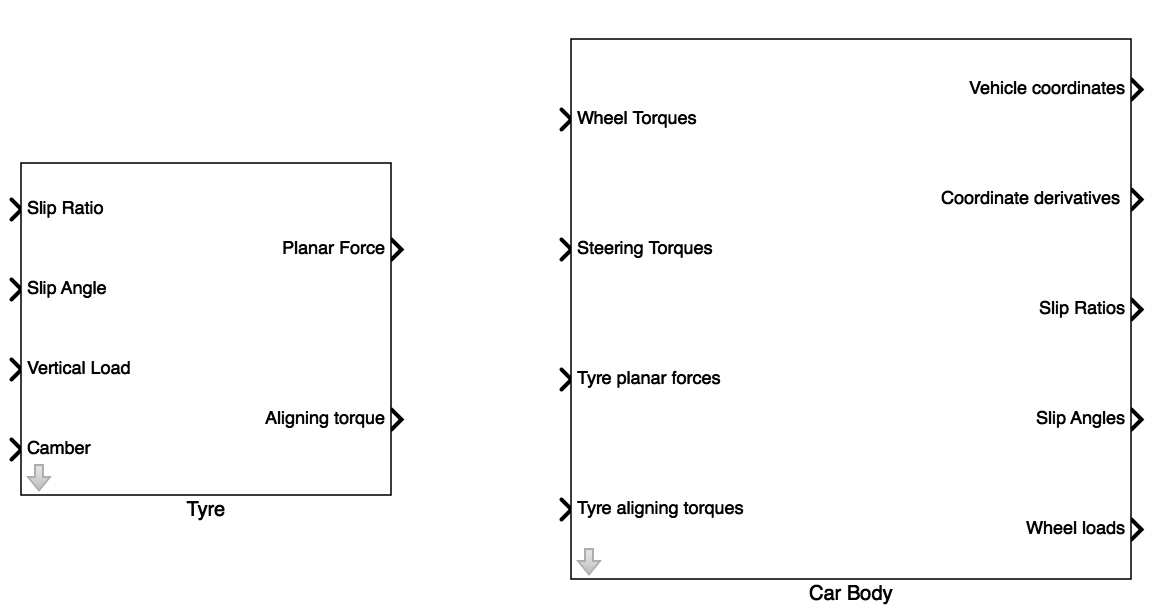
\includegraphics[scale=0.5]{images/bodyblockmask.png}
  \caption{Simulink blocks containing the tyre model and the 12DoF model.}
  \label{blocks}
\end{figure}

\section{Tyre block}

The Tyre model is implemented as a MATLAB function. The inputs are the slip ratio, the slip angle, the vertical force and the camber angle. The outputs are the horizontal force 2D vector $(F_x, F_y)$ and the aligning torque.
If all the tyres of the car are the same a single tyre block can be used to model all four wheels of the car, this is done by concantenating the inputs horizontally into a matrix. The forces corresponding to each tyre can then be extracted as columns of the outputs.
The outputs are computed by evaluating the Magic Formula equations described in \todo{cita manual adams}.
The coefficients representing the tyre for the simulations must be given in the Adams Car ".TIR" format. The format is human readable as a plaintext file, as described in \todo{adams}.
The tire model file must be located in the Matlab working directory. The name of the file can be entered in the "block mask" accessible by double clicking the block (Figure \ref{tyremask}).

\begin{figure}[ht]
  \centering
  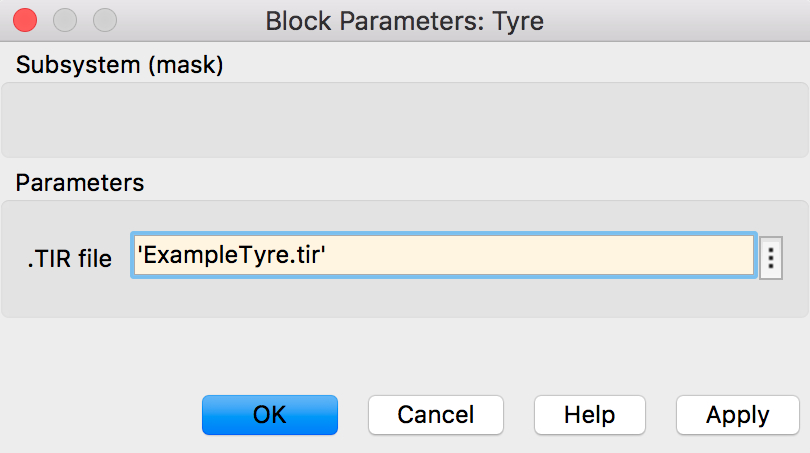
\includegraphics[scale=0.5]{images/tyremask.png}
  \caption{Simulink mask for the tyre block allows selection of the tyre model.}
  \label{tyremask}
\end{figure}

The parameters are loaded from the file into the tyre block workspace during the initialization phase by means of a script which takes advantage of the "loadTIR" function by Marco Furlan\cite{loadtir}.

Note that tyres are not simmetrical, the model used in these simulations reflects this property. For this reason care should be taken when modelling tyres on opposite sides of the car. The ".TIR" files contain a field specifying for which side the empirical coefficients were fitted. To model tyres on the other side all inputs and outputs can be redefined in a simmetrical reference system. This simply means the slip angle and camber angle signs have to be changed before entering the tyre model and the lateral force and aligning moment signs have to be changed after they are output.

\section{Vehicle Body Block}
\label{sec:bodyblock}
The internal block diagram for the 12 DoF Model is shown in figure \ref{12diag}.
\begin{figure}[ht]
  \centering
  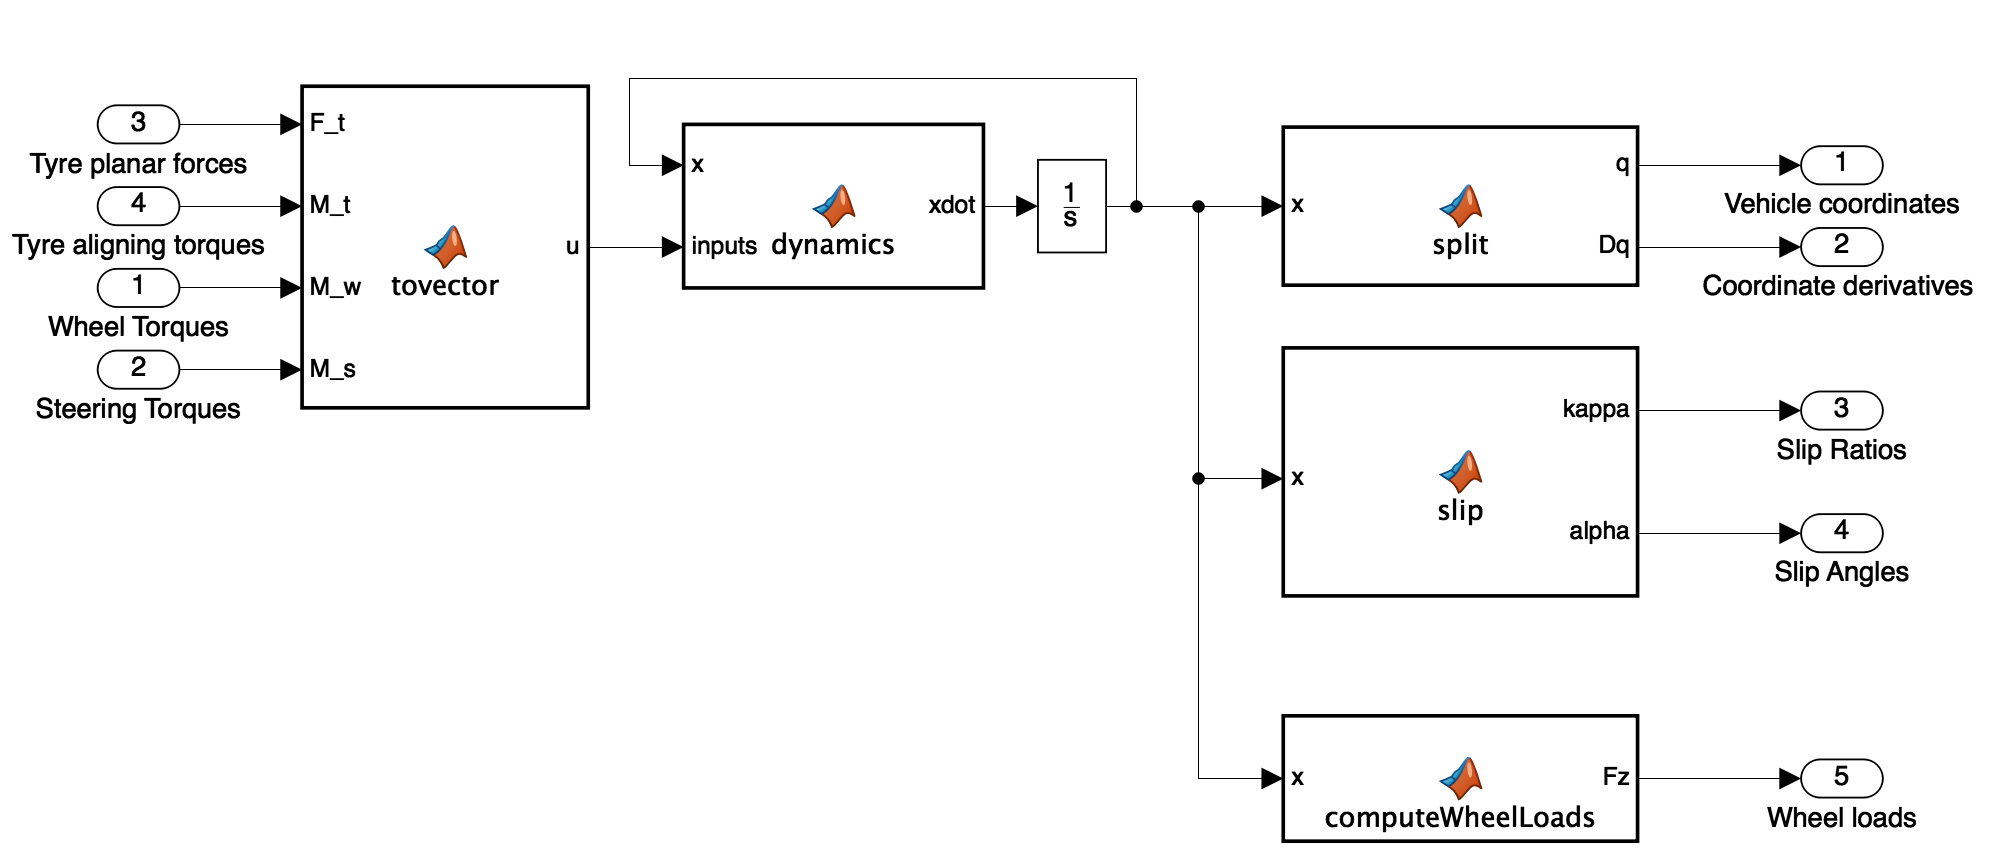
\includegraphics[width=\textwidth]{images/12dofinside.png}
  \caption{Simulink block diagram for the 12DoF model.}
  \label{12diag}
\end{figure}
The dynamics block evaluates the state space representation of the system starting from the value of the state and the inputs, yielding the state derivative $\dot x$ which is then integrated and closes it's feedback lock.
The "tovector" block simply assembles the incoming signals into the input vector for the dynamic system. The "split" block disassembles the state vector $x$ into the lagragian coordinates and their derivatives.
The "slip" block takes the vehicle coordinates as an input, calculates the contact point velocities and returns the slip angles and slip ratios.
The compute wheel loads block evaluates the vertical wheel forces using the formulas in \ref{6dofout}.
The initial state for the integrator is taken from the block mask along with the vehicle parametrization.



\begin{figure}[ht]
  \centering
  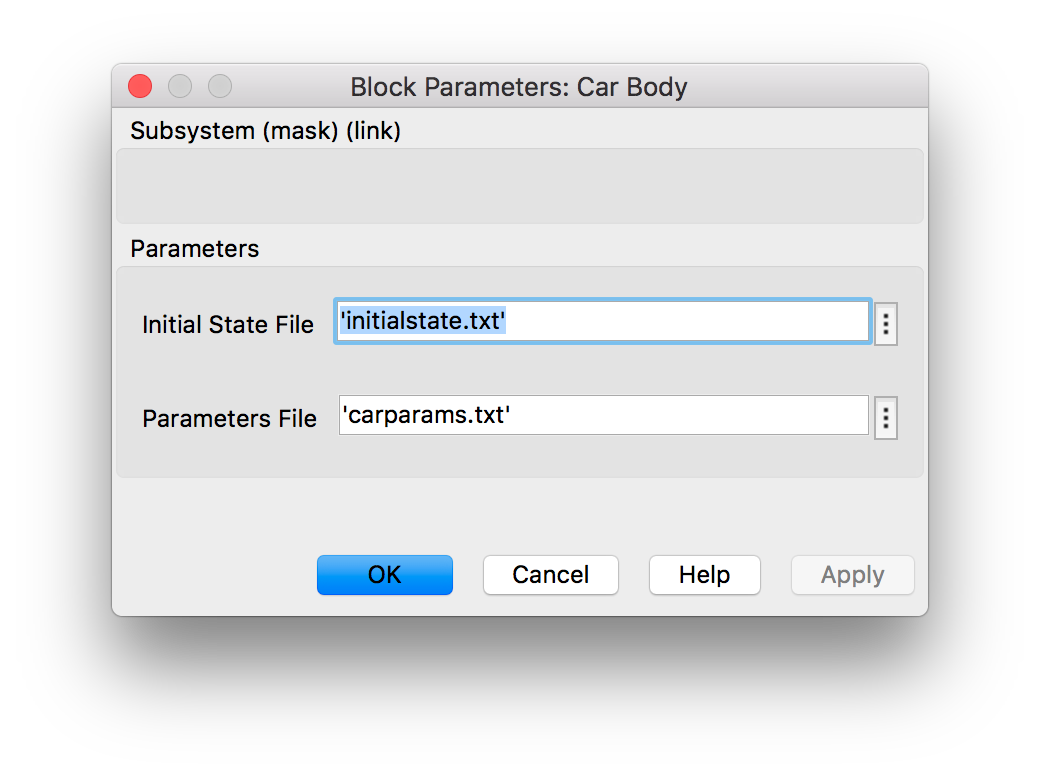
\includegraphics[width=\textwidth]{images/bodymask.png}
  \caption{Simulink block mask for the 12DoF Model.}
\end{figure}




\subsection{Parameters and initial state}

\begin{lstlisting}[caption={Parameters Declaration}]
% gravitational acceleration
syms g
% track widths
syms t_f t_r
% Front / Rear Axle Distance from CG
syms l_f l_r
% Front / Rear Roll center height
syms q_f q_r
\end{lstlisting}



\section{Top level simulation diagram}

\begin{sidewaysfigure}[ht]
  \centering
  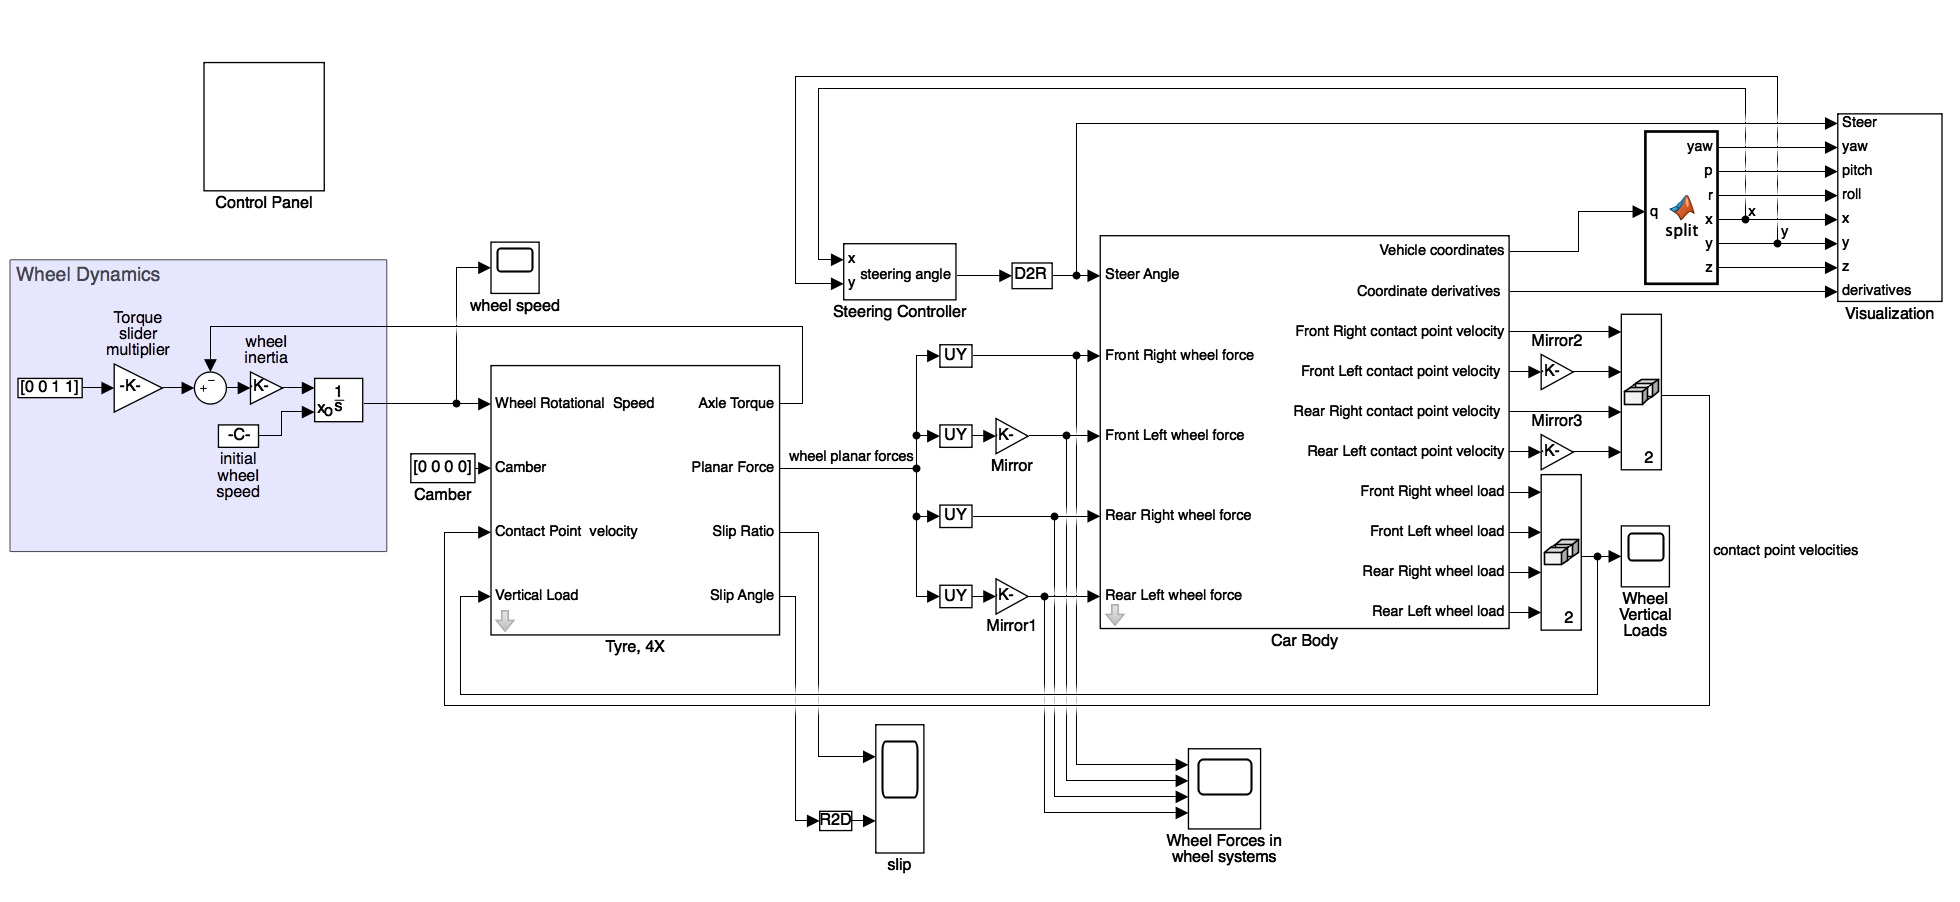
\includegraphics[width=\textwidth]{images/6dofsimulink.png}
  \caption{Vehicle response for 0.5 Hz sinusoidal steering input.}
  \label{regression}
\end{sidewaysfigure}

\chapter{Conclusion}
\label{chap:conclusion}

\begin{figure}[ht]
  \centering
  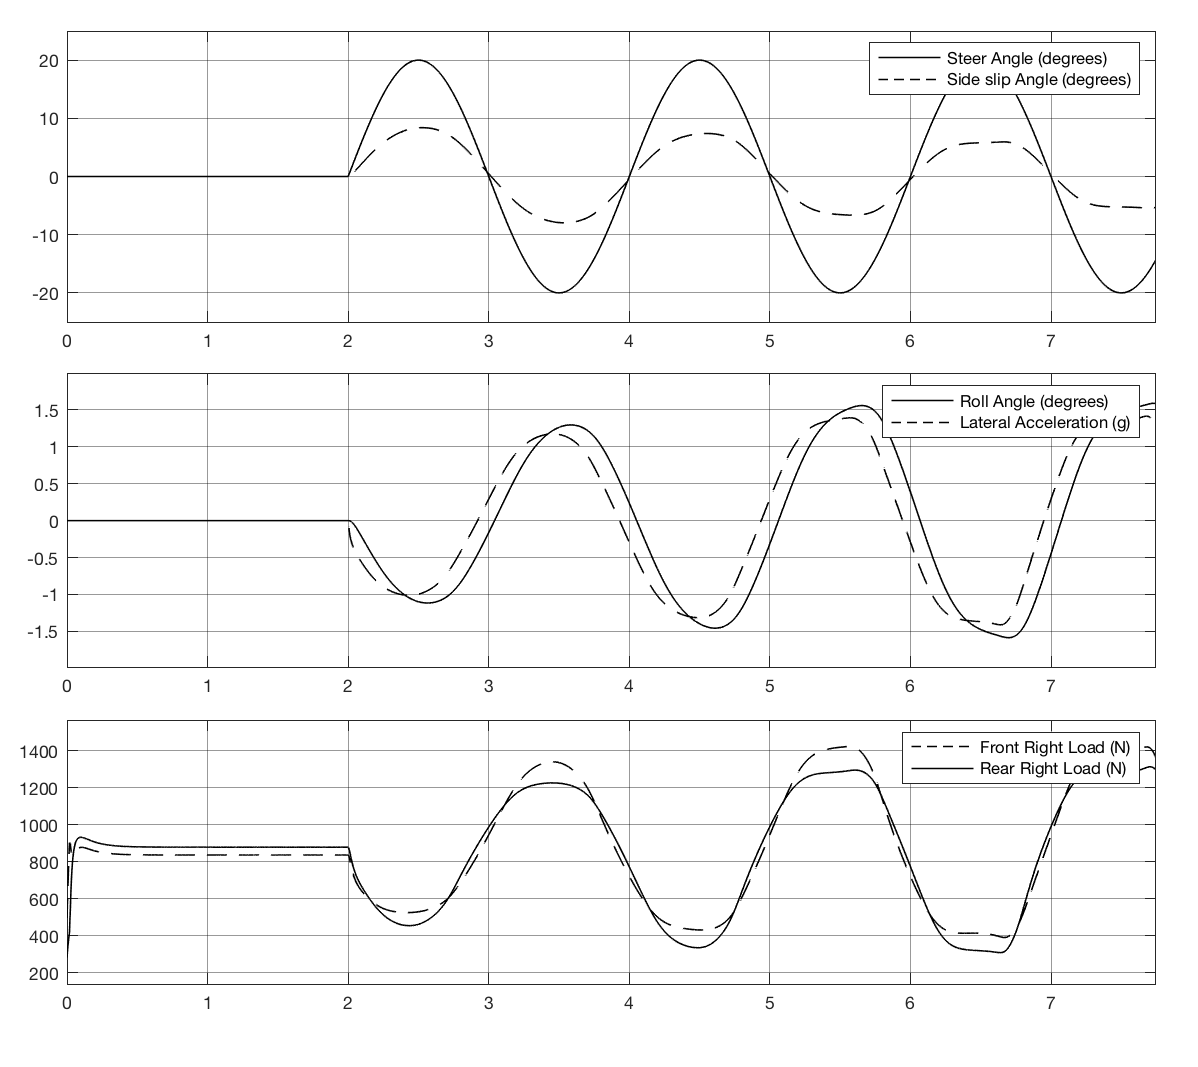
\includegraphics[scale=0.8]{figures/sine}
  \caption{Vehicle response for 0.5 Hz sinusoidal steering input.}
  \label{sine}
\end{figure}
\section{Future Work}
\label{sec:future}
\subsection{Aerodynamic effects}
\subsection{Driving algorithm}



\appendix
% INCLUSIONE APPENDICI - - PERSONALIZZARE - TENERE COERENTE CON LISTA IN ALTO
\chapter{Roll center approximation}
\label{chap:roll}

The SAE definition of roll center is

\textit{\say{The point in the transverse vertical plane through any pair of wheel centers at which lateral forces may be applied to the sprung mass without producing suspension roll}}

This definition directly relates the $P_w$ points to the roll center height.
Validity for chosen roll center approximation can be shown by modifying a generic equilibrium situation such as the one described in figure \todo{la stessa di prima} and applying a new side force $F'$ acting on the midpoint $M_F$ of $P_{FR}$ and $P_{FL}$, if the tyres are capable of generating the necessary friction forces ($F_1$ and $F_2$), the system will settle in a new equilibrium state.
The sum of vertical forces acting on the tyres does not change as it is equal to
$$
F_z := F_{z1}+F_{z2} = mg.
$$

As $F_z$ does not change, the increase in side friction force is entirely due to changes in the lateral friction coefficients, which are both supposed as being equal to $\mu_y$.

The fact that the spring systems are constrained in the vertical orientation means the horizontal forces acting at the ground contact points effect the chassis directly at the points $P_{FR}$ and $P_{FL}$ respectively.

The horizontal force balance is given by
$$
F + F' = F_1 + F_2 = \mu_y ( F_{z1} + F_{z2} ) = \mu_y mg
$$

To find the equilibrium roll angle the torque balance about point $M_F$ must be solved
$$
\frac{t_F}{2} \sin \phi (F_1-F_2) - \frac{t_F}{2} \cos \phi ( F_{z1} - F_{z2} ) - F (h_{CG}-q_F)  \cos \phi = 0
$$

substituting the friction forces yields
$$
\frac{t_F}{2} ( F_{z1} - F_{z2} ) [\mu_y \sin \phi - \cos \phi ] - F (h_{CG}-q_F)  \cos \phi = 0
$$

The vertical forces act through the springs (spring rate $k_F$) . As Hooke's law is linear, the difference between them is proportional to the difference between the spring lengths which is in turn obtained as a function of the roll angle.
$$
F_{z1} - F_{z2} = - k_F t_F \sin \phi
$$

The moment balance then becomes
$$
\mu_y k_F \frac{t_F^2}{2} \sin^2 \phi - k_F \frac{t_F^2}{2} \sin \phi \cos \phi - F(h_{CG}-q_F) \cos \phi = 0
$$

\todo{find source for roll angles in passenger cars being a few ° max} The equation may be linearized with respect to $\phi$.
$$
- k_F \frac{t_F^2}{2}  \phi  - F(h_{CG}-q_F) = 0
$$

Doing so makes the solution for $\phi$ independent of $\mu_y$, the only quantity influenced by $F'$. The height of point $M_F$ is then effectively the roll center height according to the SAE definition.

The roll rate $K_\phi$ is defined as roll angle per unit of lateral force applied to the CG \todo{find source}, applying this definition to the linearized equation gives the expression to be used to derive spring rates for the 6DoF model in order to match the roll-rate of the car.
$$
K_\phi = \frac{\phi}{F} = 2\frac{h_{CG}-q_F}{K_Ft_F^2}
$$

\chapter{Model Parameters files}
\label{chap:params}

\begin{figure}[ht]
\begin{Verbatim}
# car parameters file, variable names must match those used in carmodel.m
# all units are metric
g          9.81       # gravity
t_f        1.2        # front track
t_r        1.2        # rear track
l_f        0.8        # Front axle to CG distance
l_r        0.8        # Rear axle to CG distance
q_f        0.09       # front roll center height
q_r        0.09       # rear roll center height
h_CG       0.3        # CG height
I_f        1          # Front Steering inertia
I_r        1          # Rear steering Inertia
k_f        35000      # front virtual spring stiffness
k_r        35000      # rear virtual spring stiffness
b_f        2000       # front virtual suspension damping
b_r        2000       # rear virtual suspension damping
m          300        # sprung mass (including driver)
m_u        50         # unsprung mass
Ixx        30         # Moment of inertia about longitudinal axis (sprung only)
Iyy        60         # Moment of inertia about lateral axis (sprung only)
Izz        50         # Moment of inertia about vertical axis (sprung only)
Ixz        0          # vertical-longitudinal inertia coupling
I_u        50         # unsprung mass rotational inertia about vertical axis
r_0        0.26       # wheel radius
I_w        0.3        # wheel rotational inertia
\end{Verbatim}
\caption{Structure for the vehicle parameters file}
\label{params}
\end{figure}

\begin{figure}[ht]
\begin{Verbatim}
# initial state file, variable names must match those used in carmodel.m
# all units are metric SI
y         0        # initial yaw
p         0        # initial pitch
r         0        # initial roll
x_CG      0        # initial CG coordinates
y_CG      0        # initial CG coordinates
z_CG     -0.3      # initial CG coordinates
delta_f   0        # initial front steer angle
delta_r   0        # initial rear steer angle
gamma_fr  0        # initial wheel angular position (FR)
gamma_fl  0        # initial wheel angular position (FL)
gamma_rr  0        # initial wheel angular position (RR)
gamma_rl  0        # initial wheel angular position (RL)
Dy        0        # initial yaw rate
Dp        0        # initial pitch rate
Dr        0        # initial roll rate
Dx_CG     1        # initial CG velocity wrt inertial frame
Dy_CG     0        # initial CG velocity wrt inertial frame
Dz_CG     0        # initial CG velocity wrt inertial frame
Ddelta_f  0        # initial front steering rate
Ddelta_r  0        # initial rear steering rate
Dgamma_fr 0        # initial wheel speed (FR)
Dgamma_fl 0        # initial wheel speed (FL)
Dgamma_rr 0        # initial wheel speed (RR)
Dgamma_rl 0        # initial wheel speed (RL)
\end{Verbatim}
\caption{Structure for the initial vehicle state file}
\label{init}
\end{figure}

\chapter{Matlab code}
\section{Generalized forces function}
\label{sec:genforces}
\lstinputlisting[label=lst:12code]{code/genforces.m}
\section{12DoF Model generation script}
\label{sec:12dofcode}
\lstinputlisting[label=lst:12code]{code/carmodel.m}

%%%%%%%%%%%%%%%%%%%%%%%%%%%%%%%%%%%%%%%%%%%%%%%%%%%%%%%%%%%%%%%

% BIBLIOGRAFIA
\addcontentsline{toc}{chapter}{\refname}
\nocite{*}
\printbibliography

\end{document}
